\chapter{Wykorzystane oprogramowanie}
\section{Eclipse}
\subsection{Rys historyczny}
W 2001 roku pojawił się na rynku mało znany projekt typu \emph{otwarte oprogramowanie} – \emph{Eclipse 1.0}. Program ten został opisany jako ,,zintegrowane środowisko deweloperskie do wszystkiego i do niczego w szególności''\ref{eclipsearticle}. W założeniu nie miał to być kolejny zestaw narzędzi, a w pełni skalowanle i rozszerzalne środowisko programistyczne. Razem z programem, udostępniono szereg narzędzi dla programistów, umożliwiających rozwijanie projektu. Początkowo Eclipse powstał tylko po to, by dowieść, że można zbudować środowisko rozszerzalne w tak dużym zakresie. Dzięki społeczności, bardzo szybko środowisko to rozwinęło się na wiele języków programowania (ponad 1500 narzędzi w \emph{http://marketplace.eclipse.org} na początku stycznia 2014 roku).

Typowy wizerunek programisty otwartego oprogramowania ukazuje bezinteresownego programistę, nocami pracującego nad poprawą błędów i implementacją własnych pomysłów. W Eclipse, początkowe fragmenty kodu były napisane przez programistów firmy \emph{IBM}. Pracownicy ci dostawali pełne wynagrodzenie za pracę nad otwartym projektem, odpowiadaniem na pytania społeczności, naprawą błędów. Początkowy wkład w rozwój Eclipse miały firmy takie jak \emph{Borland}, \emph{IBM}, \emph{Merant}, \emph{QNX Software Systems}, \emph{Rational Software}, \emph{RedHat}, \emph{SuSE}, a także \emph{TogetherSoft}. Firmy te mogły dzięki temu liczyć na wypuszczenie na rynek programów komercyjnych bazujących na tym środowisku. 

Pierwotnie Eclipse składał się z głównych elementów: \emph{Eclipse Platform}, \emph{Eclipse JDT} oraz \emph{Eclipse PDE}. Eclipse Platform stanowił bazę, środowisko programistyczne. JDT to skrót od \emph{Java Devevelopment Tools} - była to pierwsza większa wtyczka, umożliwiająca zarządzanie kodem Java. Jest ona dostępna do dziś, oczywiście w dużo bardziej zaawansowanej formie niż na początku. Ostatni element, PDE (\emph{Plug-in Development Environment}) to narzędzie do rozwijania środowiska Eclipse. Oferuje ono szereg domyślnych wtyczek, zawiera kreatory tworzenia nowych modułów, a także ogromną i wyczerpującą dokumentację na temat całego środowiska.

Na początku Eclipse było znane jako czysta platforma, dziś jest to zaawansowane środowisko programistyczne z ponad 1500 mniejszymi i większymi rozszerzeniami. W Internecie można znaleźć narzędzia i wtyczki do Eclipse umożliwające pisanie i testowanie kodu niemal w każdym języku programowania.

\subsection{Platforma}

Program Eclipse zbudowany jest w języku \emph{Java}, wymaga więc zainstalowanej Javy na komputerze użytkownika.  Całe środowisko składa się osobnych wtyczek współpracyjących ze sobą, oraz rdzenia samego programu (ang. \emph{Eclipse kernel}). Wtyczka to nic innego, jak plik \emph{JAR} z manifestem, określającym zachowanie i przeznaczenie modułu. W manifestach zawierane są również informacje na temat zależności między wtyczkami:

Przykład zależności między wtyczkami opisanych w pliku plugin.xml
\begin{verbatim}
<requires>
	<import plugin="org.apache.xerces"/>
	<import plugin="org.eclipse.core.resources"/>
	<import plugin="org.eclipse.update.core"/>
	:       :        :
	<import plugin="org.eclipse.text" export="true"/>
	<import plugin="org.eclipse.ui.workbench.texteditor" export="true"/>
	<import plugin="org.eclipse.ui.editors" export="true"/>
</requires>
\end{verbatim}

By zachęcić twórców do rozwijania środowiska Eclipse, wymyślono tzw. \emph{Extension Points}. Extension Points to instrukcje informujące Eclipse, jakich klas użyć do rozszerzenia elementów takich jak okna, menu kontekstowe, kreatory. Korzystając z tych punktów można domyślne elementy podmienić własnymi, bardziej rozbudowanymi modułami. Dzięki takiemu rozwiązaniu, rdzenną aplikację można niemal w nieograniczony sposób dostosować do swoich potrzeb.\ref{ana_structure}

\JP{czy ten przykład służy czemukolwiek?}
\begin{verbatim}
<extension-point id="decorators" name="%ExtPoint.decorators"
                 schema="schema/decorators.exsd"/>
\end{verbatim}

\begin{figure}[h]
  \centering
    \includegraphics{img/custom-window.png}
    \caption{Dodatkowa zakładka Plan Browser}
    \label{ana_structure}
\end{figure}

Dobrym przykładem jest tutaj całkiem popularne środowisko deweloperskie \emph{Aptana Studio}. Aplikacja ta została zbudowana całkowicie na rdzeniu Eclipse, można więc zauwazyć pewne podobieństwa w układzie okien, modułowości. Mimo podobieństw jest jednak zupełnie inna, ukierunkowana na jedną gałąź programowania – \emph{Web Development}\JP{ten termin angielski na pewno nie jest potrzebny}. Nie wszyscy twórcy potrzebują jednak tworzyć całkowicie odrębne oprogramowanie. Eclipse SDK przychodzi z szeregiem domyślnych modułów, takich jak dekoratory, edytory tekstu, paski narzędzi i nawigatory\JP{znam słowo nawigatorzy, ale ono odnosi się do żeglugi. Co to są nawigatory?}. Każdy z tych modułów może zostać zastąpiony własnym lub rozszerzony o pewne funkcjonalności.

\subsection{Perspektwywy}
Pojęcie perspektywy jest ważnym elementem środowiska Eclipse. Perspektywy pozwalają na zarządzanie konkretnym układem okien służących do wykonania określonego działania. Każde większe rozszerzenie posiada własną perspektywę, która posiada specyficzne dla danego języka programowania opcje i funkcje. Utworzenie tzw. perspektywy pozwala w środowisku Eclipse na płynne przełączanie między perspektywami dla różnych języków, w zależności od wybranego pakietu podstawowego i rozszerzeń zainstalowanych w Eclipse.

\section{ANTLR}
ANTLR (ang. \emph{ANother Tool for Language Recognition}) jest generatorem
analizatorów leksykalnych i składniowych \cite{antlr}.

Narzędzie przetwarza opisy gramatyk języków formalnych w postaci 
zbliżonej do notacji
 Backusa-Naura\JP{tu cytowanie}. Na podstawie specyfikacji generowany jest kod analizatora.
Językami programowania wspieranymi przez ANTLR są między innymi C, C\#, Java
i Python.

Istotną zaletą oprogramowania jest jego prostota użycia. Wygenerowany kod 
jest czytelny i \JP{może zostać łatwo dołączony do tworzonej} łatwo można go dołączyć do własnej aplikacji. Postać plików
wejściowych jest podobna dla wszystkich rodzajów analizatorów. Dodatkowo
istnieją narzędzia wspierające projektowanie i implementację gramatyk
formalnych z wykorzystaniem ANTLR. Należy do nich ANTLRWorks, będące
zintegrowanym środowiskiem programistycznym. Zawiera ono edytor strukturalny,
zintegrowany program do usuwania błędów i moduł do wizualizacji struktur 
danych powstających podczas translacji.

ANTLR został opublikowany wraz z kodem źródłowym na licencji BSD\JP{URL}. Projekt jest
aktywnie rozwijany. Wiele programów zawiera analizatory wygenerowane za pomocą
ANTLR, np. Hibernate\JP{URL}, Jython\JP{URL} i Netbeans\JP{URL}.

\subsection{Przetwarzanie języków formalnych}
Języki formalne, w tym języki programowania, są opisane zbiorem zasad określającym
ich składnię i semantykę. Analiza języka formalnego polega na sprawdzeniu zgodności
danych wejściowych ze specyfikacją języka oraz na wyodrębnieniu części składniowych.
Ponadto podczas analizy mogą zostać wykonane operacje działające na danych zgodnie
z~ich znaczeniem określonym przez reguły semantyczne \cite{compilers}.

\JP{a może zrezygnować z tego wypunktowania i napisać coś pokroju: Wyodrębnia się trzy fazy analizy. Zależności między nimi przedstawione są na rysunku \ref{antlr_phases}}
Wyodrębnia się trzy fazy analizy:
\begin{enumerate}
\item \emph{Analizę leksykalną}.
\item \emph{Analizę składniową}.
\item \emph{Analizę semantyczną}.
\end{enumerate}

\begin{figure}[h]
  \centering
    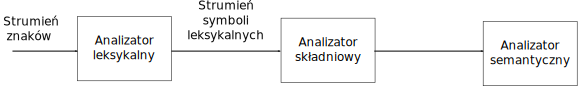
\includegraphics[width=\textwidth]{img/antlr_phases.pdf}
    \caption{Fazy analizy języka formalnego}
    \label{antlr_phases}
\end{figure}

Zależności pomiędzy fazami przedstawia rysunek \ref{antlr_phases}. 

Podczas analizy leksykalnej dane wejściowe są traktowane jako strumień znaków, który
jest odczytywany od strony prawej do lewej. Znaki są grupowane w \emph{symbole leksykalne}, czyli
ciągi posiadające określone znaczenie. Analiza składniowa ma na celu zgrupowanie 
symboli leksykalnych w hierarchiczne struktury,
mające pewne znaczenie.\JP{Z tego fragmentu nie wynika, żeby analiza leksykalna czymś różniła się od składniowej: tak czy siak na końcu są struktury mające znaczenie, co niczego nie mówi} Analiza semantyczna przetwarza dane zgodnie z ich znaczeniem
opisanym przez reguły semantyczne. W~tej fazie zbierane są informacje zawarte w danych.

Reguły języka mogą być opisane językiem naturalnym lub w sposób sformalizowany.
Jednym z formalizmów, odzwierciedlającym hierarchiczną strukturę konstrukcji językowych,
jest \emph{gramatyka bezkontekstowa} \JP{tu cytowanie}. Składa się ona z czterech elementów:

%Pytanie nieuniknięto powtórzenia skłów w definicji
\begin{itemize}
\item Zbioru symboli leksykalnych zwanych \emph{symbolami terminalnymi} lub \emph{terminalami}.
\item Zbioru symboli \emph{nieterminalnych}.
\item Zbioru \emph{produkcji}. Każda produkcja składa się z symbolu nieterminalnego,
  zwanego lewą stroną produkcji, strzałki i ciągu symboli zwanego prawą stroną produkcji.\JP{Czy ta strzałka to jest zaczerpinęta z jakiejś mądrej książki?}
\item Wyznaczonego \emph{symbolu startowego}.
\end{itemize}

Gramatyka \emph{wyprowadza ciąg symboli leksykalnych}, jeżeli wychodząc 
od symbolu startowego i zamieniając symbole nieterminalne na ciągi znajdujące 
się po prawych stronach produkcju, można otrzymać dany ciąg. Sposób, w~jaki
można wyprowadzić dany napis obrazuje \emph{drzewo wyprowadzania}. W~korzeniu drzewa wyprowadzania
znajduje się symbol startowy. Dzieci wierzchołka reprezentującego symbol nieterminalny
zawierają symbole z prawej strony produkcji użytej do jego zastąpienia.

\JP{Proszę przepisać bezosobowo. Ja chyba nie do końca rozumiem czym jest requirementName, bo potem pojawia się :strips jako konkretny przykład. Dobrze by też było, żeby ten przykład był trochę bardziej rozbudowany, bo potem rysunek \ref{antlr_ast} wygląda drętwo.}
\paragraph{Przykład 4.1}
Rozpatrzmy przykład konstrukcji języka PDDL reprezentującej listę wymagań domeny lub problemu.
Składa się ona z otoczonych nawiasami okrągłymi symbolu \texttt{:requirements} oraz
ciągu symboli oznaczających nazwy wymagań. Symbolami terminalnymi są 
\textbf{(}, \textbf{)}, słowo kluczowe \textbf{:requirements} i 
\textbf{requirementName} reprezentujący nazwę wymagania. Poniższa gramatyka opisuje
składnię takiego wyrażenia:

\begin{itemize}
\item requirementsList $\rightarrow$ \textbf{(} \textbf{:requirements} R
\item R $\rightarrow$ \textbf{requirementName} \textbf{)}
\item R $\rightarrow$ \textbf{requirementName} \textbf{R}
\end{itemize}

Dla napisu postaci \texttt{(:requirements :strips)} zostanie
wygenerowany strumień symboli leksykalnych \textbf{( :requirements requirementName )}.
Drzewo wyprowadzania tworzone podczas analizy składniowej jest przedstawione 
na rysunku \ref{antlr_example}

\begin{figure}[h!]
  \centering
    \includegraphics[width=0.7\textwidth]{img/antlr_example.pdf}
    \caption{Drzewo wyprowadzania dla przykładu 12\JP{tu chyba inny numer?}}
    \label{antlr_example}
\end{figure}

\subsection{Metoda LL(*)}
Główną zaletą gramatyk bezkontekstowych jest możliwość automatycznego generowania programów
wykonujących analizę leksykalną i składniową na podstawie gramatyki\JP{tu cytowanie}.

Narzędzie ANTLR generuje analizatory leksykalne i składniowe dla pewnego podzbioru
gramatyk formalnych. Elementy tego podzbioru nazwane są gramatykami LL(*). Metoda 
analizy stosowana w generowanych analizatorach nazwana jest analizą LL(*). 

Analizatory LL(*) należą do klasy analizatorów LL. Wykorzystują one
analizę zstępującą i metodę zejść 
rekurencyjnych. Każdemu nieterminalowi zdefiniowanemu w specyfikacji gramatyki
odpowiada procedura lub metoda\JP{nie bardzo rozumiem to procedura lub metoda. Nie wystarczy jedno z tych słów?}. 

Analiza\JP{jaka? składownia? zstępująca?}, polegająca na konstrukcji drzewa
wyprowadzenia, rozpoczyna się od korzenia. Związany z nim jest symbol 
startowy gramatyki. W każdym kroku analizy wykonywane są następujące czynności:
\JP{Skoro mówimy o drzewie, to chyba jednak właściwszym tłumaczeniem byłyby wierzchołki, a nie węzły}
\begin{enumerate}
\item Wybierany jest pierwszy w porządku, zdefiniowanym przez
  przeszukiwanie wgłąb, węzeł $V$ zawierający symbol nieterminalny $A$.\JP{skąd się wzięło to $A$?}
\item Wybierana jest produkcja mająca po lewej stronie symbol $A$.
\item Jako dzieci węzła $V$ dodawane są węzły związane z symbolami znajdującymi się po prawej
  stronie produkcji z punktu 2.
\end{enumerate}

Typy analizatorów należących do klasy LL różnią się sposobem wyboru produkcji w punkcie 2. 
Analizatory LL(*) są analizatorami przewidującymi. Podejmują one decyzję na
podstawie nieprzetworzonych symboli leksykalnych w strumieniu wejściowym. Liczba
tych symboli nie jest ograniczona. W celu przeglądania strumienia wejściowego 
,,w przód'' tworzone są automaty skończone mogące zawierać cykle.

W odróżnieniu od tradycyjnych gramatyk LL, w~gramatykach LL(*) prawe strony
produkcji dla jednego nieterminala mogą mieć ten sam prefiks. Nie ma więc 
konieczności lewostronnej faktoryzacji, co znacznie ułatwia tworzenie
gramatyk.\JP{Termin lewostronna faktoryzacja musi zniknąć albo być wyjaśniony, bo teraz nie wiadomo o co chodzi.}

\subsection{Abstrakcyjne drzewa składniowe}
% Analizę semantyczną języka opisanego gramatyką bezkontekstową można 
% sprowadzić do obliczania wartości atrybutów przyporządkowanych symbolom
% znajdującym się w drzewie wyprowadzanie. Produkcjom przypisywane są 
% wówczas reguły określające wartości atybutów. Takie podejście 

Formą pośrednią przekazywaną pomiędzy analizatorem składniowym, a semantycznym
może być \emph{abstrakcyjne drzewo składniowe}. Jest to skondensowana postać drzewa
wyprowadzania, składająca się
wyłącznie z węzłów reprezentujących symbole wejściowe. Węzły
wewnętrzne reprezentują słowa kluczowe i operatory, liście -- argumenty.
Abstrakcyjne drzewo składniowe dla przykładu 1\JP{znowu coś z tym numerem jest nie tak} jest przedstawione na rysunku 
\ref{antlr_ast}.

\begin{figure}[h!]
  \centering
    \includegraphics[scale=0.8]{img/antlr_ast.pdf}
    \caption{Abstrakcyjne drzewo składniowe dla przykładu 1\JP{tak jak pisałem wyżej: ten rysunek jest nie dość fascynujący}}
    \label{antlr_ast}
\end{figure}

%Przykład drzewa

Możliwe jest ręczne tworzenie drzewa składniowego za pomocą odpowiednich
reguł semantycznych. Takie podejście proceduralne jest opisane w \cite{compilers}.

Narzędzie ANTLR wspiera tworzenie drzew składniowych. Dodanie
odpowiedniej opcji w specyfikacji analizatora składniowego powoduje automatyczne
wygenerowanie struktury. Poza tym, specyfikacja analizatora składniowego
 może zawierać elementy deklaratywne wpływające na kształt drzewa.


Przetwarzanie abstrakcyjnego drzewa składniowego podczas analizy semantycznej
sprowadza się do jego przechodzenia. Można do tego wykorzystać analizator drzewowy. \JP{Czy drzewowy jest na pewno poprawnym terminem po polsku? Może warto, żeby pojawiła się angielska wersja w nawiasie}
Jest to podprogram generowany przez
ANTLR na podstawie specyfikacji, tak jak analizator składniowy lub leksykalny.
Wprowadzenie analizatorów drzewowych wyróżnia ANTLR na tle innych generatorów
 parserów.  \JP{Czy to się czymś różni od wzorca Visitor? Jeżeli tak, to czym? Jeżeli nie, to warto o tym napisać.}

\subsection{Pliki wejściowe}

Pliki wejściowe ANTLR posiadają rozszerzenie \texttt{.g}. Zawierają one specyfikację
analizatora leksykalnego, składniowego, drzewowego lub połączoną specyfikację
analizatorów leksykalnego i składniowego. 

Specyfikacja analizatorów składa się z listy produkcji, definiujących symbole,
 sekcji opcji konfiguracyjnych oraz kodu dodawanego do generowanego
pliku źródłowego.

W przypadku plików zawierających połączoną specyfikację analizatorów, występuje
podział symboli ze względu na pierwszą literę ich nazwy.
 Symbole, których nazwa rozpoczyna się wielką literą uznawane są
za symbole terminalne. W ich definicjach mogą występować literały i inne
symbole terminalne. Na podstawie reguł definiujących symbole terminalne
tworzony jest analizator leksykalny. Pozostałe reguły tworzą analizator
składniowy.

\JP{Tu bym widział jakiś krótki przykład takiego pliku i/lub odwołanie do odpowiedniego dodatku z omówionym przynajmniej fragmentem takiego kodu ze stworzonego projektu.}
